\documentclass[]{article}
\usepackage[utf8]{inputenc}
\usepackage[margin=1.0in]{geometry}
\usepackage{amsmath, amsfonts}
\usepackage{tikz}
\usepackage[english]{babel}
\usepackage{amsthm}
\usepackage{enumitem}
\usepackage{graphicx}
\usepackage{float}
\usepackage[backend=biber]{biblatex}
\usepackage{hyperref}
\usepackage{subcaption}

\newtheorem{theorem}{Theorem}
\newtheorem{definition}{Definition}
\newtheorem{lemma}{Lemma}
\newtheorem{corollary}{Corollary}[theorem]
\renewcommand{\theenumi}{\Alph{enumi}}

\newcommand{\bd}{\textbf}
\newcommand{\del}{\nabla}
\newcommand{\by}{\times}
\newcommand{\R}{\mathbb R}
\newcommand{\C}{\mathbb C}
\newcommand{\M}{\mathcal M}
\newcommand{\Borel}{\mathcal B_{\mathbb R}}
\newcommand{\dprime}{^{\prime\prime}}
\newcommand{\tprime}{^{\prime\prime\prime}}
\newcommand{\x}{\mathbf x}
\newcommand{\y}{\mathbf y}
\newcommand{\z}{\mathbf z}
\renewcommand{\v}{\mathbf v}
\renewcommand{\S}{\mathbb S}
\renewcommand{\u}{\mathbf u}
\newcommand{\innerprod}[2]{\left\langle #1\,, #2 \right\rangle}
\addbibresource{bibliography}


\title{Additional Proofs to Kirsch and Grinberg's  "The Factorization Method for Inverse Problems"}
\date{}
\author{Kale Stahl}

\begin{document}
		
		%Makes fancy title
		\makeatletter
		\begin{center}
			{\centering \Large \bd \@title}\\
			\vspace{.5cm}
			{\large \@author}
			\vspace{.25cm}
		\end{center}
		\makeatother
		\begin{abstract}
			The goal of this project is to provide additional proof and explanation of the factorization of the far-field operator for the inverse scattering problem. We seek to prove that the far field operator can indeed be factored into an auxiliary and Herglotz operator. We will then prove that utilizing this factorization yields a unique solution to the inverse scattering problem and implement this method numerically.
		\end{abstract}
		\tableofcontents
		
		\section{Introduction}		
			This project will be devoted to studying the Factorization method for inverse scattering problems proposed by Andreas Kirsch and Natalia Grinberg in \cite{kirschgrinberg2008}. It will focus on the simplest cases seen in the first chapter of this book. We will consider the scattering of time-harmonic plane waves by an object $D$ which is modeled by the Dirichlet boundary condition on the boundary $\Gamma = \partial D$ of $D$. We consider acoustic waves, which are characterized by the Helmholtz equation. We will omit analysis of the direct scattering problem, and focus only on additional analysis to the factorization methods used to solve the inverse scattering problem. We will first show that the far field operator can be decomposed into the solution operator, and then we will prove the actual factorization of the far field operator. Once this is done, we will prove the uniqueness of the inverse problem utilizing properties of the factorization method and provide numeric reconstructions.
		\section{The Factorization Method}
			
			\subsection{Equality of the Far-Field and Solution Operators}
				Our goal is to prove an auxiliary theorem in the factorization of the far-field operator. Before we do this, we define the far field operator as follows.
				\begin{definition}[Far-Field Operator]
					Define the far-field operator $F:L^2(\mathbb S^2) \to L^2(\mathbb S^2)$ as
					\begin{equation}	
						(Fg)(\hat x) = \int\limits_{\mathbb S^2}u^\infty(\hat x, \theta)g(\theta)\, ds(\theta) \qquad \hat x\in \S^2
					\end{equation}
					where $u^\infty(\hat x)$ is the far field pattern of $u$ defined as
					\begin{equation}
						u^\infty(\hat x) = \int\limits_\Gamma\left[u(y)\frac{\partial }{\partial u(y)}e^{-ik\hat x\cdot y} - \frac{\partial u(y)}{\partial u}e^{-ik\hat x\cdot y}\right]\, ds(y) \qquad \hat x\in \S^2
					\end{equation}
				\label{def:F}
				\end{definition}
				When considering the inverse scattering problem, this operator contains the known data. We wish to use this operator to obtain explicit characterizations about the unknown domain $D$. 
				We then will define an operator to which this far-field operator decomposes into, which is based on the Herglotz operator.
				\begin{definition}
					\label{def:H}
					Define $H: L^2(\mathbb S^2) \to H^{1/2}$ as
					\begin{equation}
						-(Hg)(\hat x) = -\int\limits_{\mathbb S^2}g(\theta)e^{ikx\cdot \theta}\,ds(\theta) \qquad x\in \Gamma
					\end{equation}
					note that this is the trace on $\Gamma$ of the Herglotz wave function with density $g$.
				\end{definition}
				\begin{definition}
					\label{def:G}
					Let the data-to-pattern operator $G: H^{1/2}(\Gamma)\to L^2(\S^2)$ be defined by $Gf =m v^\infty$ where $v^\infty \in L^2(\S^2)$ is the far field pattern of the solution $v$ to the exterior Dirichlet problem with boundary data $f\in H^{1/2}(\Gamma)$, meaning that $v\in H^1_{\text{loc}}(\R^3\setminus\bar D)$ solves 
					\begin{equation}
						\begin{cases}
							\Delta v + k^2v = 0 &\text{outside }D\\
							v = f & \text{on } \Gamma
						\end{cases}
					\end{equation}
				\end{definition}
				Using these definitions, we will prove the following theorem involving the elementary factorization of the far-field operator into the solution operator $G$ and the auxiliary operator $H$.
				\begin{theorem}
					Let $F$ and $H$ be the operators defined above. $G: H^{1/2} \to L^2(\mathbb S^2)$ be the solution operator. We then have 
					\begin{equation}
						Fg = -GHg
					\end{equation}
				\end{theorem}
				\begin{proof}
					For some data $f_\theta(x)= -e^{ik\theta \cdot x}$, the $G$ operator
					\begin{equation}
						Gf_\theta(x) = u^\infty(\hat x, \theta)
					\end{equation}
					We note that 
					\begin{equation}
						(Hg)(x) = \int g(\theta)e^{ikx\cdot \theta}\, ds(\theta) 
					\end{equation}
					Applying the solution operator $G$, we have 
					\begin{align}
						(GHg)(x) &= G\int\limits_{\mathbb S^2} g(\theta)e^{ikx\cdot \theta}\,ds(\theta)\\
						&= \int\limits_{\mathbb S^2} g(\theta)Gf_\theta\, ds(\theta)\\
						&=  \int\limits_{\mathbb S^2}u^\infty(\hat x, \theta)g(\theta)\, ds(\theta)\\
						(GHg)(x) &= -Fg
					\end{align}
					Now, we need to show that we can indeed pull the operator inside of the integral. To do this we first must decompose $f$ into $f^+$ and $f^-$ where $f = f^+-f^-$ such that $f^+$ and $f^-$ are positive semidefinite. This is to say that $f^+$ is equivalent to $f$ when $f>0$ and 0 otherwise and $f^-$ is equivalent to $f$ when $f<0$ and 0 otherwise. Now, by the Approximation Theorem we can pick a sequence $\{f^+_{n}\}$ of monotone increasing positive simple functions such that $f^+_{n}\to f^+$ as $n \to \infty$. We can write each term in this sequence as 
					\begin{equation}
						f^+_{n} = \sum^n_{i=0}\alpha_i(x)\chi_{E_i}(\theta)
					\end{equation} 
					Where $\alpha_i$ are some sequence of constants and $\chi_{E_i}$ are characteristic functions of some set $E_i$. Thus, we see by the summation definition of the Lebesgue integral, we see that the $G$ operator can be pulled inside and then by the Monotone Convergence theorem, we can switch the integral and limit for $f^+$. We can apply the same linearity to $f^-$ by the linearity of the Lebesgue integral. So then with this shown, we indeed have 
					\begin{equation}
						Fg = -GHg 
					\end{equation}
				\end{proof}
			\subsection{Factorization of the Far-Field Operator}
			\begin{definition}
				\begin{equation}
					S\varphi(x) := \int\limits_\Gamma \Phi(x, y) \varphi(y)\, ds(y), \qquad x \in \Gamma
				\end{equation}
				with 
				\begin{equation}
					\Phi(x, y) = \frac{e^{ik|x-y|}}{4\pi|x-y|}, \qquad x, y \in \R^3, \quad x\neq y
				\end{equation}
			\end{definition}
			\begin{lemma}
				We have that $v= S\varphi$ is a solution to the Hemholtz equation. Moreover, $H^\ast \varphi$ is the far-field pattern for the $v = S\varphi$ function.
			\end{lemma}
			\begin{proof}
				Define $\Phi(x, y)$ as the Green's function for the three dimensional Hemholtz equation. We begin by noting for a fixed $y\neq x$, we have
				\begin{equation}
					\Delta_x \Phi(x, y) + k^2 \Phi(x, y) = \delta(x-y)
				\end{equation}
				We can multiply both sides by $\varphi(y)$ and integrate over $\partial D$ to see
				\begin{equation}
					\int\limits_{\partial D}\Delta_x \Phi(x, y)\varphi(y) + k^2 \Phi(x, y)\varphi(y)\, ds(y) = \int\limits_{\partial D}\delta(x-y)\varphi(y)\, ds(y)
				\end{equation}
				Since $x\neq y$, the right-hand side goes to 0 and we have
				\begin{equation}
					\int\limits_{\partial D}\Delta_x \Phi(x, y)\varphi(y)\, ds(y) + k^2\int\limits_{\partial D}\Phi(x, y)\varphi(y)\, ds(y) = 0
				\end{equation}
				By linearity of the Lebesgue integral, and the fact that $\Delta_x$ is independent of the integral, we are able to pull it out of the integral. To prove this fact, we must first consider the limit definition of the derivatives included in the $\Delta_x$ operator. Considering a single derivative with respect to $x_1$ we have
				\begin{equation}
					\frac{\partial }{\partial x}\Phi(x, y) = \lim_{(\delta x_1)_n \to 0}\frac{\Phi(x+ (\delta x_1)_n, y) - \Phi(x, y)}{(\delta x_1)_n}
				\end{equation}
				Define $(\delta x_1)_n = \{\frac{1}{n}\}^{\infty}_{n =1}$ so then $(\delta x_1)_n\to 0 $ as $n \to \infty$. We will now apply Lesbesgue's Dominated Convergence theorem. We first note that $ \left|\frac{\Phi(x+ (\delta x_1)_n, y) - \Phi(x, y)}{(\delta x_1)_n}\right|$ is bounded from above by $|\Phi(x, y)|$ which is in $L^2(\partial D)$. Thus, by the Dominated convergence Theorem we have
				\begin{equation}
					\int\limits_{\partial D}\frac{\partial }{\partial x_1}\Phi(x, y)\, ds(y) = \int\limits_{\partial D}\lim_{(\delta x_1)_n \to 0}\frac{\Phi(x+ \delta x_n, y) - \Phi(x, y)}{\delta x_n}\, ds(y) =  \frac{\partial }{\partial x_1}\int\limits_{\partial D}\Phi(x, y)\, ds(y)
				\end{equation}
				The same argument can be repeated for both the second derivative of $x_1$ and the two derivatives of $x_2$, meaning the entire $\Delta_x$ operator can be pulled outside the integral.
				Finally, by applying Definition 1, we see that
				\begin{equation}
					\Delta_xS\varphi(x)+ k^2S\varphi(x) = 0
				\end{equation}
				Meaning that $v = S\varphi(x)$ is indeed a solution to the Hemholtz equation.				
				
				Next we will show that $v = S\varphi(x)$ satisfies the necessary radiation condition. We note that our radiation condition is given by
				\begin{equation}
					\frac{\partial v}{\partial r} - ikv = \mathcal O(r^{-2}) \qquad r = |x| \to \infty
				\end{equation}
				We will begin by applying the radiation condition to $\Phi (x, y)$, seeing
				\begin{equation}
					\frac{\partial}{\partial |x|}\Phi (x, y) - ik \Phi (x, y) = \mathcal O(|x|^{-2})
				\end{equation}
				multiply both side by $\varphi(y)$ and integrating over $\partial D$, we have
				\begin{equation}
					\int_{\partial D}\frac{\partial}{\partial |x|}\Phi (x, y)\varphi(y)\, ds(y) - \int_{\partial D}ik \Phi (x, y)\varphi(y)\, ds(y) = \int_{\partial D}\mathcal O(|x|^{-2})\, ds(y)
				\end{equation}
				By the same argument as previous, we can pull out the derivative, seeing
				\begin{equation}
					\frac{\partial}{\partial r}S\varphi(x) - ikS\varphi(x) = \mathcal O(|x|^{-2})
				\end{equation}
				We see that the right-hand side will go to zero as the integral is over the boundary and any small terms will vanish. Thus, $v= S\varphi(y)$ satisfies our radiation condition.
				Finally we will show that $H^\ast \varphi$ is the far-field pattern. We start by noting
				\begin{equation}
					\Phi^\infty(\hat x, y) = e^{-ik\hat x\cdot y}
				\end{equation}
				and in general we have
				\begin{equation}
					\varphi(\hat x, y, k) = \frac{e^{ik|x|}}{|x|}\left[ \varphi^\infty(\hat x, y, k) + \mathcal O(|x|^{-2})\right] 
				\end{equation}
				We can then see
				\begin{align}
					S\varphi(\hat x) &= \frac{e^{ik|x|}}{|x|}\left[ (S\varphi)^\infty(\hat x) + \mathcal O(|x|^{-2})\right] \\
					&= \int\limits_{\partial D} \Phi(\hat x, y)\varphi(y)\, ds(y)\\
					&= \int\limits_{\partial D}\frac{e^{ik|x|}}{|x|}\left[ \Phi^\infty(\hat x, y) + \mathcal O(|x|^{-2})\right] \varphi(y)\, ds(y)\\
					&= \frac{e^{ik|x|}}{|x|}\left[ \int\limits_{\partial D} \Phi^\infty(\hat x, y)\varphi(y)\, ds(y) + \mathcal O(|x|^{-2})\int\limits_{\partial D} \varphi(y)\, ds(y)\right] \\
					&= \frac{e^{ik|x|}}{|x|}\left[ \int\limits_{\partial D} e^{-ik\hat x\cdot y}\varphi(y)\, ds(y) + \mathcal O(|x|^{-2})\right] \\
					&= \frac{e^{ik|x|}}{|x|}\left[ H^\ast \varphi(y) + \mathcal O(|x|^{-2})\right] \\
				\end{align}
				From here we can conclude that indeed $	(S\varphi)^\infty(\hat x) =H^\ast \varphi(\hat x)$ and we are finished.
			\end{proof}
			\begin{theorem}
				If $k^2$ is not a Dirichlet Eigenvalue of $-\Delta$ in $D$ we arrive at the factorization
				\begin{equation}
					F = H^\ast S^{-1}H
				\end{equation}
			\end{theorem}
			\begin{proof}
				We will first calculate $H^\ast$ explicitly. We see for some inner product $\innerprod{\cdot}{\cdot}$ and some $f \in L^2(\mathbb S^2)$ and $g\in H^{1/2}(\partial D)$ we have 
				\begin{equation}
					\innerprod{Hf}{g}_{H^{1/2}} = \innerprod{f}{H^\ast g}_{L^2}\label{Hstar}
				\end{equation}
				Define
				\begin{equation}
					\innerprod{f(x)}{g(x)}_{H^{1/2}(\partial D)} = \int\limits_{\partial D} \overline{g(x)}f(x)\, ds(\theta)
				\end{equation}
				and
				\begin{equation}
					\innerprod{f(x)}{g(x)}_{L^2(\mathbb S^2)} = \int\limits_{\mathbb S^2}\overline{g(x)}f(x)\, ds(\theta)
				\end{equation}
				Using (\ref{Hstar}) we can calculate $H^\ast$, seeing
				\begin{align}
					\innerprod{Hf}{g}_{H^{1/2}} &=  \int\limits_{\partial D} \overline{g(x)}Hf(x)\, ds(\theta)\\
					 &=  \int\limits_{\partial D} \overline{g(x)} \int\limits_{\mathbb S^2}f(\theta)e^{ikx\cdot \theta}\, ds(\theta) \, ds(\theta)\\
					 &=  \int\limits_{\partial D}  \int\limits_{\mathbb S^2}\overline{g(x)e^{-ikx\cdot \theta}}f(\theta)\, ds(\theta) \, ds(\theta)\\
					 &=  \int\limits_{\mathbb S^2}\int\limits_{\partial D}  \overline{g(x)e^{-ikx\cdot \theta}}\, ds(\theta)f(\theta) \, ds(\theta)\\
					 &= \innerprod{f}{H^\ast g}_{L^2}
				\end{align}
				So then we have
				\begin{equation}
					H^\ast g(\theta) = \int\limits_{\partial D}g(x)e^{-ikx\cdot \theta}\, ds(\theta)
				\end{equation}
				By Lemma 1, we know that $H^\ast = GS$ since $GS$ yields the far field pattern of $S$. Thus we have,
				\begin{equation}
					 -H^\ast S^{-1}Hg = -GSS^{-1}H = -GIH = -GH
				\end{equation}
				So then by Theorem 1 we know that $-GH = F$ so then $-H^\ast S^{-1}H = F$ and we are finished.\\
			\end{proof}
		\section{Uniqueness of the Solution to the Factorization Method}
			The following theorem, which appears in \cite{kirschgrinberg2008} without proof, is used to prove the uniqueness of the solution to the inverse scattering problem. The proof of the theorem in \cite{coltonkress2013} uses more general tools such as Rellich's lemma, but we can utilize what we have already proved about the factorization method along with general notions about the inverse scattering problem to arrive at a rather elegant proof. We also need to establish some general facts about the far-field pattern before we can arrive at this proof. The following Lemma, taken from \cite{kirschgrinberg2008}, helps to show the uniqueness of the far-field pattern with respect to the domain.
			\begin{lemma}
				\label{lemma:test-function}
				Let $G$ be defined as in Definition \ref{def:G}. For any $z\in \R^3$ define the test function $\phi_z \in L^2(\S^2)$ by 
				\begin{equation}
					\phi_z(\hat x) := e^{-ik\hat x\cdot z}, \qquad \hat x\in \S^2
				\end{equation}
				Then $\phi_z$ belongs to the range of $G$ if and only if $z\in D$.
			\end{lemma}
			\begin{proof}
				We first take some $z\in D$ and define
				\begin{equation}
					v(x) := \Phi(x, z) = \frac{e^{ik|x-z|}}{4\pi |x-z|}, \quad x\notin D
				\end{equation}
				and $f|_\Gamma$. Then $f \in H^{1/2}(\gamma)$. Theh the far-field pattern of $v$ is given by 
				\begin{equation}
					v^\infty(\hat x)
				\end{equation}
			\end{proof}
			This allows us to associate a test function with our domain and characterize whether or not a point exists within the domain. With this defined, we can state the following uniqueness theorem:
			\begin{theorem}
				\label{theorem:uniqueness}
				For a fixed wavenumber $k>0$ the far field patterns $u^\infty(\hat x, \theta)$ uniquely determine the shape of the scattering object $D$. This means that if there are two objects $D_1$ and $D_2$ with corresponding far field patterns $u_1^\infty(\hat x, \theta)$ and $u_2^\infty)(\hat x, \theta)$ respectively, then $u_1^\infty(\hat x, \theta)=u_2^\infty)(\hat x, \theta)$ implies that $D_1=D-2$.
			\end{theorem}
			\begin{proof}
				To prove this, we first begin by supposing there are two objects, $D_1$ and $D_2$ such that their far-field patterns coincide. 
			\end{proof}
		\section{Numeric Simulations}
			This section will show the Factorization Method implemented with simulated data and its ability to reconstruct various objects. MATLAB code samples for implementing the factorization method are found in \cite{potthast2015}. The code used to create these simulations can be found on my \href{https://github.com/KaleStahl/Honors-Project}{Github}.
			
			 We begin by taking three differently shaped scattering objects and use the factorization method to reconstruct them. In Figure \ref{fig:noiseless}, we have a kite, a circle, and an ellipse.
			\begin{figure}[h]
				\centering
				\begin{subfigure}{.3\textwidth}
					\centering
					\includegraphics[width = \textwidth]{Numeric Simulations/Images/Circle-Reconstructed}
					\caption{Circle shaped scattering object}
				\end{subfigure}
				\begin{subfigure}{.3\textwidth}
					\centering
					\includegraphics[width = \textwidth]{Numeric Simulations/Images/ellipse-Reconstructed}
					\caption{Ellipse shaped scattering object}
				\end{subfigure}
				\begin{subfigure}{.3\textwidth}
					\centering
					\includegraphics[width = \textwidth]{Numeric Simulations/Images/kite-Reconstructed}
					\caption{Kite shaped scattering object}
				\end{subfigure}
				\caption{Reconstructions of scattering objects with no noise in data.}
				\label{fig:noiseless}
			\end{figure} 
			We can see that the reconstructions are rather accurate. The reconstructions in Figure \ref{fig:noiseless} have data which is has no "noise", that is, the data used to reconstruct the object is representative of the exact data expected from the scattering problem.
			
			In practical applications this is not always the most feasible assumption, as real data is often "noisy". This noise can be caused by various factors, but yields data which varies from the expected perfect data. To simulate this, we will add randomly generated Gaussian noise to the far-field operator used to solve the inverse problem. This noise is scaled such that the matrix norm of the noisy far-field operator and the exact far-field operator differ by a given percent, which we will represent our "noise level" in the figures. The estimate used in the noise generation technique to do this is found in \cite{hansen1988}. We see in Figure \ref{fig:circlenoise} circles, in Figure \ref{fig:ellipsenoise} ellipses, and Figure \ref{fig:kitenoise} kites, all with various levels of noise. Obviously the reconstructions are much less accurate than their noiseless counterparts, but they are still able to reconstruct the general shape of the original object.
			\begin{figure}[h]
				\centering
				\begin{subfigure}{.3\textwidth}
					\centering
					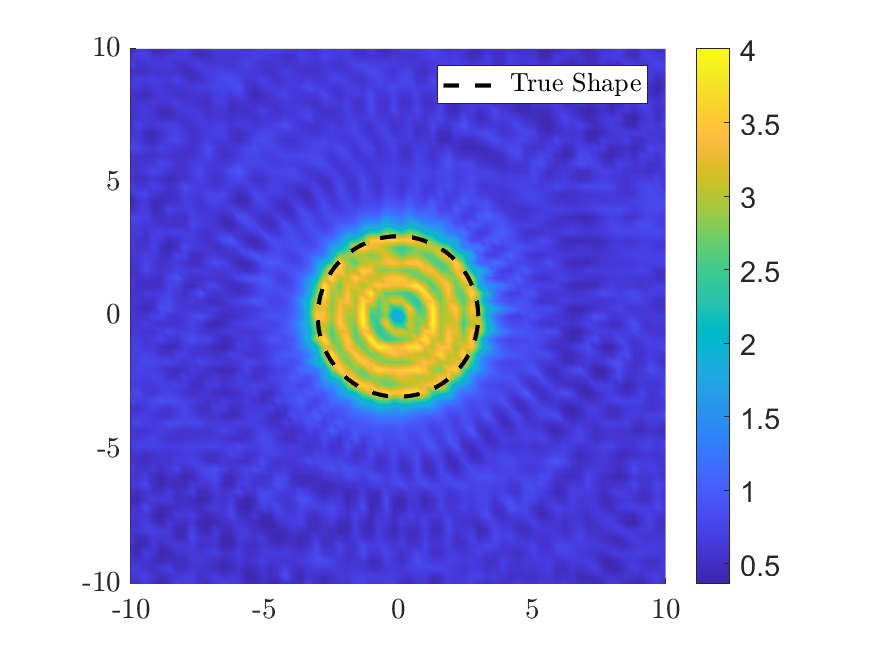
\includegraphics[width = \textwidth]{Numeric Simulations/Images/circle-10-noise-reconstructed}
					\caption{Circle with 10\% added noise.}
				\end{subfigure}
				\begin{subfigure}{.3\textwidth}
					\centering
					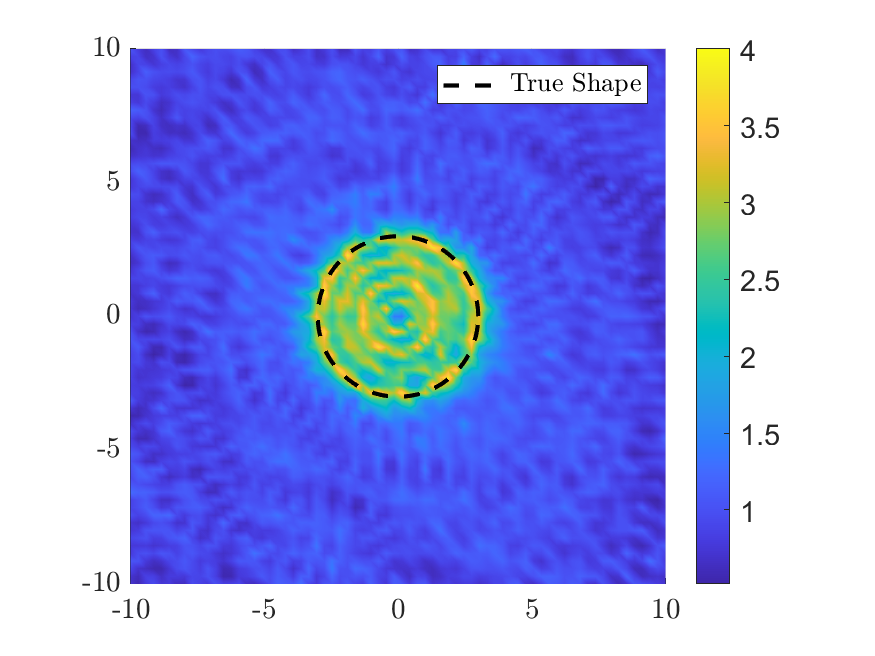
\includegraphics[width = \textwidth]{Numeric Simulations/Images/circle-20-noise-reconstructed}
					\caption{Circle with 20\% added noise.}
				\end{subfigure}
				\begin{subfigure}{.3\textwidth}
					\centering
					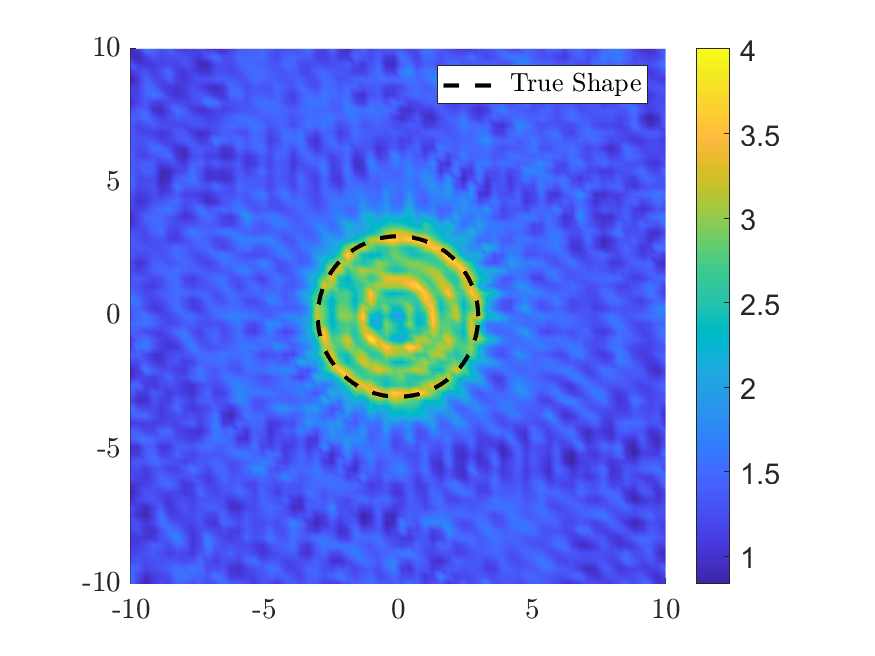
\includegraphics[width = \textwidth]{Numeric Simulations/Images/circle-40-noise-reconstructed}
					\caption{Circle with 40\% added noise.}
				\end{subfigure}
				\caption{Reconstructions of circular objects with various levels of noise in data.}
				\label{fig:circlenoise}
			\end{figure} 
			\begin{figure}[h]
				\centering
				\begin{subfigure}{.3\textwidth}
					\centering
					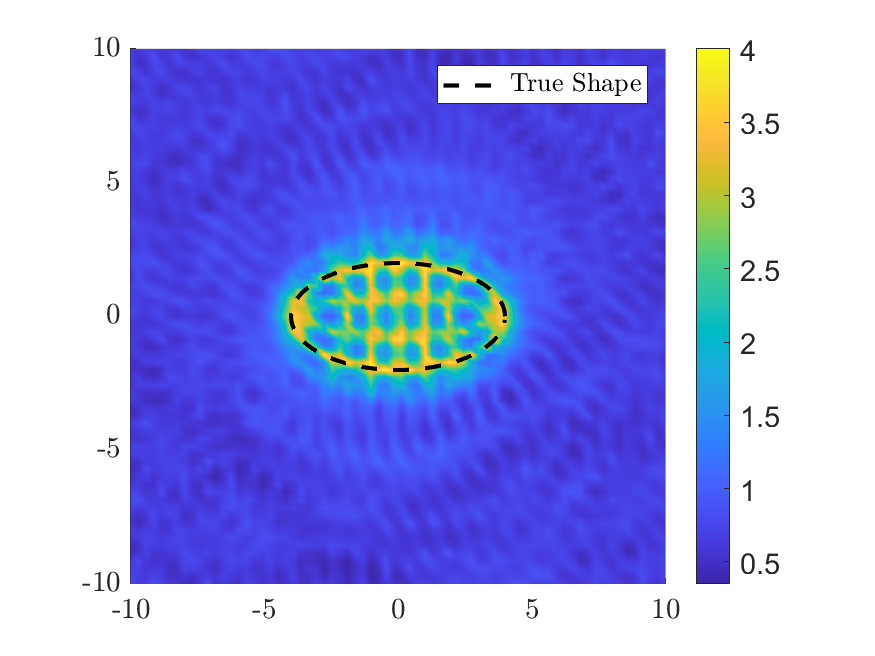
\includegraphics[width = \textwidth]{Numeric Simulations/Images/ellipse-10-noise-reconstructed}
					\caption{Ellipse with 10\% added noise.}
				\end{subfigure}
				\begin{subfigure}{.3\textwidth}
					\centering
					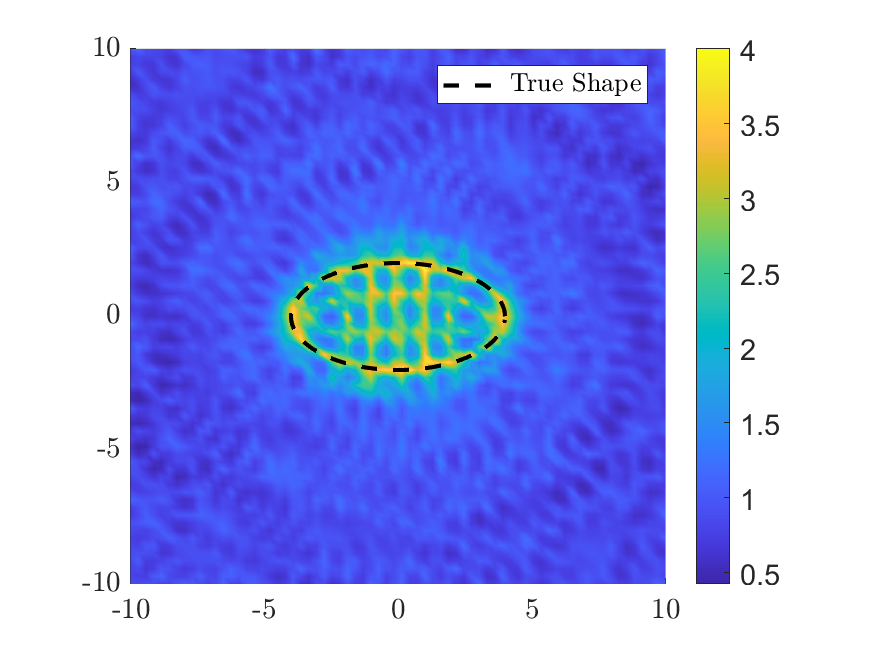
\includegraphics[width = \textwidth]{Numeric Simulations/Images/ellipse-20-noise-reconstructed}
					\caption{Ellipse with 20\% added noise.}
				\end{subfigure}
				\begin{subfigure}{.3\textwidth}
					\centering
					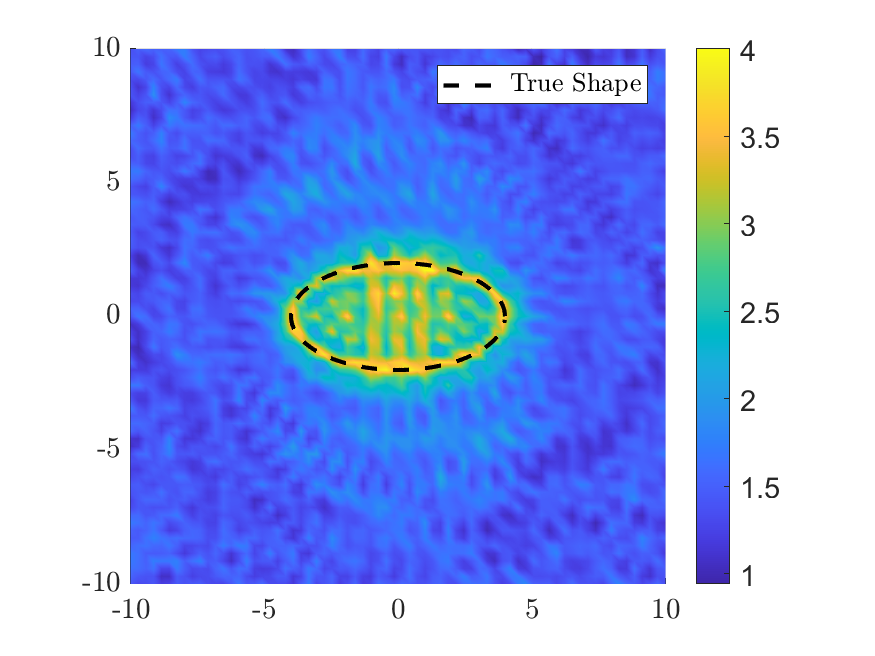
\includegraphics[width = \textwidth]{Numeric Simulations/Images/ellipse-40-noise-reconstructed}
					\caption{Ellipse with 40\% added noise.}
				\end{subfigure}
				\caption{Reconstructions of ellipses with various levels of noise in data.}
				\label{fig:ellipsenoise}
			\end{figure}
			\begin{figure}[h]
				\centering
				\begin{subfigure}{.3\textwidth}
					\centering
					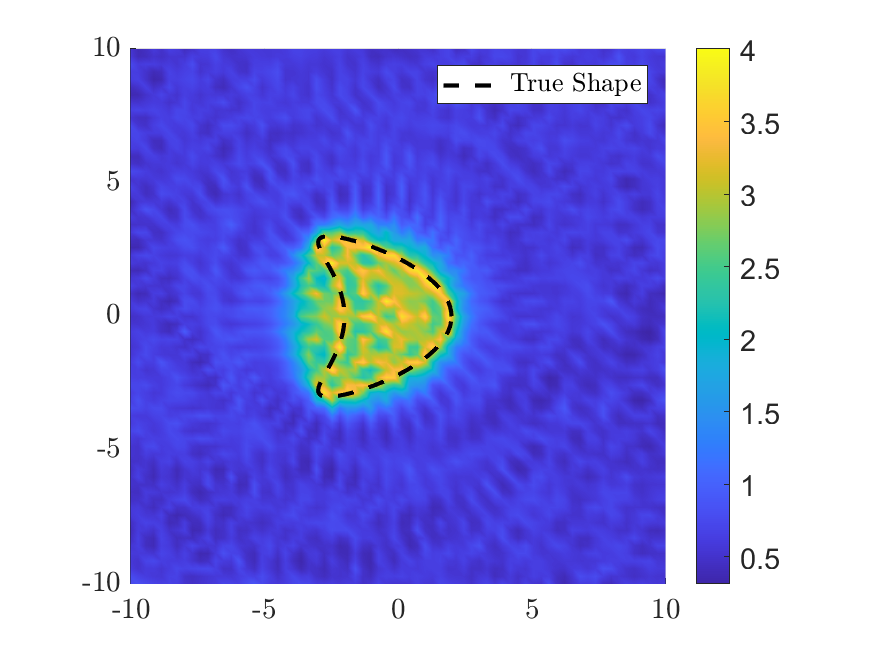
\includegraphics[width = \textwidth]{Numeric Simulations/Images/kite-10-noise-reconstructed}
					\caption{Kite with 10\% added noise.}
				\end{subfigure}
				\begin{subfigure}{.3\textwidth}
					\centering
					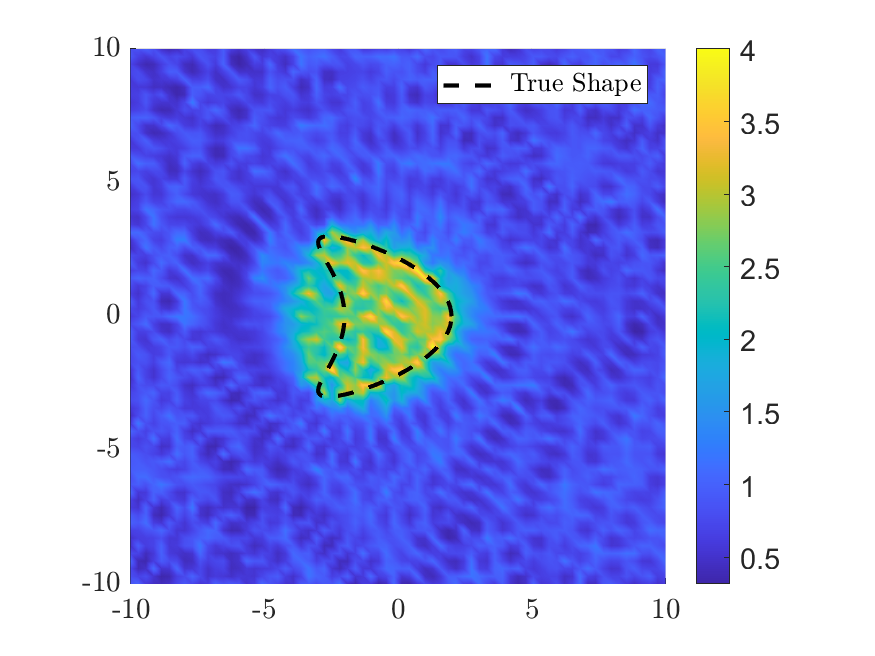
\includegraphics[width = \textwidth]{Numeric Simulations/Images/kite-20-noise-reconstructed}
					\caption{Kite with 20\% added noise.}
				\end{subfigure}
				\begin{subfigure}{.3\textwidth}
					\centering
					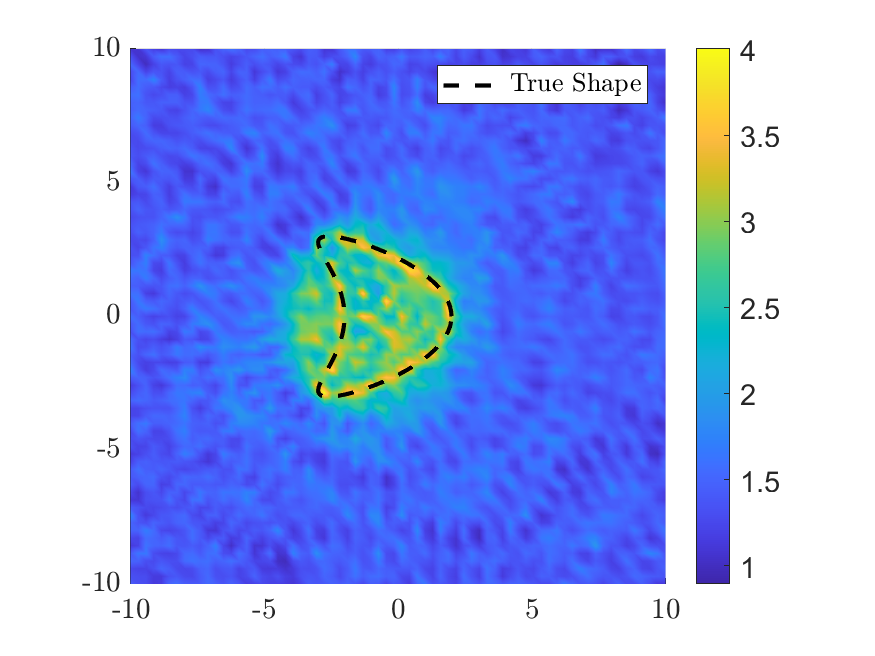
\includegraphics[width = \textwidth]{Numeric Simulations/Images/kite-40-noise-reconstructed}
					\caption{Kite with 40\% added noise.}
				\end{subfigure}
				\caption{Reconstructions of kites with various levels of noise in data.}
				\label{fig:kitenoise}
			\end{figure} 
		\printbibliography
			
\end{document}
